\section{Metal Artifact Reduction}

When we do a CT, if there is a object with a great electrical density, the final image is corrupted. This happens because these object obstruct the way of photons, so only a small number of photons, that have high energy, arrive on the sensors, then the measure is inconsistent.

These objects are in general metals, like prosthesis and peacemaker. So we call this phenomenons of Metal Artifact.

Metal Artifact Reduction is a process where the goal is reduce the error caused by the metal. There is a lot of different ways to resolve this problem. One way is interpret all measures that was altered due to the metal as lack of date. So we can use the others date to estimate them.

A large number of algorithms do the estimate through interpolation. But how interpolate? How identify the corrupt and incorrupt date? Due to the nature of CT is mandatory interpret the image not only on the 'Cartesian domain' but on the 'Radon domain' too. The 'Radon domain' is a good tool because each point represent uniquely a measure. So if we know which measures are incorrect, we can discovery, on the Radon domain, exactly which point are corrupted or not. Knowing these points we are promptly to apply any interpolation algorithm.

One way to identify the incorrect measure is discovering where is the metal on the Cartesian domain and then apply the Radon transform on these points. See a example on the figure \eqref{metal_radon}.

\begin{figure}[h]
\centering
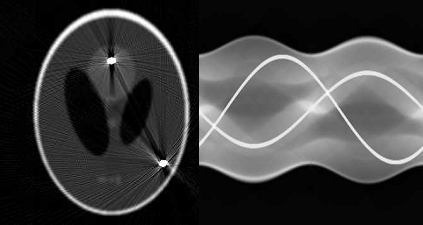
\includegraphics[scale=0.8]{img/metal_radon}
\caption{{The metallic part is the pixel with greater white intensity: On the left the image on Cartesian coordinate, on the right the sinogram (Radon Transform)}}\label{metal_radon}
\end{figure}

After identify which measures is incorrect and consequently which points on 'Radon domain' is corrupted, we can interpolate the date on the 'Radon domain' and then transform the result to the 'Cartesian domain', so we obtain the recovered image.

\subsection{Interpolation Methods}
There is a lot different ways to interpolate a data: linear interpolation, polynomial interpolation, using finite elements, minimizing a variation function,respecting a partial differential equation and so on. On the next topics we will do a brief explain on two methods, linear interpolation and the method of Bertalmio at el, which relies on the solution of a partial difference equation.

\subsection{Linear}
This method consist in interpolate all the project respect to $\theta$. In other words, for each $\theta$ we have a segment $X_d(\cdot,\theta)$ composed by cleaned and corrupted interval. The interval where the date is corrupted is restored using linear functions that connects its extremes, that are reliable data.

\begin{figure}[h]
\centering
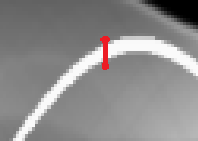
\includegraphics[scale=1]{img/LI}
\caption{Linear Interpolation, the red line on the sinogam represent the changed pixel and the interpolation extremes}\label{LI}
\end{figure}

\subsection{Method of Bertalmio at el}

This approach is based on interpreter the Radon transform as a image and then apply the techniques of image inpainting. Image inpainting is the process of reconstructing lost or deteriorated parts of images.

The Bertalmio at el. method is inspired on the work of art restorer. The main point is that the structure surrounding the deteriorated area are continued inside the gap. So the contour lines are drawn as extensions of the contour lines that touch the edge of the domain.

Furthermore, the properties of the contour lines inside the deteriorated domain, like color and smoothness, is determined by the properties that this contour line have on the edge of the domain.

In mathematics terms, the contour lines is represented by $u(x; y) = c $, where $u$ is the grey intensity. Then the direction of the contour line is $\nabla^\bot u$ and the smoothness is defined by $\Delta u$.

The Laplacian is a good estimate of smoothness because it has a large value when the variation is high and a small value when the region is regular.
Furthermore, the laplacian is related to the border in the images. So, when we propagate the laplacian we are prolonging the borders.

Therefore, we need propagate the $\Delta u$ over $\nabla^\bot u$ until arrive in a stationary condition.

The equations that describe the propagation is 
\begin{equation}\label{inpainting}
u_t =\nabla u \cdot \nabla \Delta u
\end{equation}
and is possible add a diffusion term ( $\nu\nabla\cdot(g(|\nabla u|)\nabla u)$ ) in order to obtain a smother image.

The stationary condition is reached when $u^*$ (the solution) satisfy \[\nabla^\bot u^* \cdot \nabla \Delta u^* = 0,\] because in this condition the contour lines of $u^*$  and the $\Delta u^*$ are parallels. So, there aren't anything more to propagate.

The equation \eqref{inpainting} says how the image behave inside of the deteriorated domain. Obviously, on the border of the domain $u^*$ need be equal to the imagine outside of the domain. Thus, The edge conditions can be translate by 
\[\begin{cases} u^*=u & \partial D  \\
		\nabla^\bot u^*  = \nabla^\bot u  & \partial D \\ \end{cases} \]


\subsubsection{Analogy between fluid and image}

Consider the Navier Stoker Equations for a incompressible viscous fluid.
\[\begin{cases} v_t+v\cdot\nabla v - \nu\Delta v + \nabla p = 0 & D  \\
		\nabla v  =  0 &  D \\ \end{cases} \]

Is possible prove that, in the bidimensinal case of incompressible constrains, exit a flow function $\Psi$ in such way $v=\nabla\Psi$.

Further, we can describe the Navier Stoker Equation with the vorticity $\omega$ instead of use $v$.

So,
\[\omega_t + v\cdot\nabla\omega - \nu\Delta\omega=0,\]
but,
\[\omega = \nabla\times v = \nabla\times\nabla^\bot\Psi = \Delta\Psi\]
thus,
\begin{equation}\label{vortice}
\omega_t + \nabla^\bot\Psi\cdot\nabla\Delta\Psi - \nu\Delta\Delta\Psi=0
\end{equation}

Now, is possible to see that the equation \eqref{inpainting} is analogy to the equation \eqref{vortice}, considering stationary conditions ($\omega_t=0$) and non viscous fluid ($\nu=0$),therefore we can do the  do a parallel between fluid and image, where

\begin{table}[h]
\centering
\begin{tabular}{c c c c}
\hline\hline
Fluids                             &  Image \\
\hline
Fluid flow function $\Psi$       &  Image Intensity $u$ \\
velocity $v=\nabla^\bot\Psi$       &  direction isolines of $u$,$\nabla^\bot u$ \\
vorticity $\omega$                 &  smoothness $\omega=\Delta u$ \\
viscosity $\nu$                    &  diffusivity $\nu$   \\
\hline
\end{tabular}
\end{table}

Thus, if we resolve a problem of NS, we are automatically resolving a problem of image inpainting. Moreover, numerical solutions of the Navier and Stockes problems are well known.

A important point to get in consideration is when and why use the diffusion term.

The diffusivity work like a stabilization, because without it, the resolution methods normally diverge, but using this term the solutions change. So, to minimize the error and to guaranty the convergence we can choose a expression like this, with $k$ as parameter:
\[\nu(\Vert\nabla^\bot u\Vert)=\frac{1}{1+\frac{\Vert\nabla^\bot u\Vert}{k}}\]

Thereby, when we have a high gradient of $u$, the diffusion is negligible in order to preserve the image's edge.

\subsection{Fusion Method}

After we do the Metal Artifact Reduction, in some cases, in exchange of remove the artifact, some pieces of the image are corrupted, pieces that are important to understand the image.

If these pieces were on the original image, a method called fusion based prior image can be use to recover these piece that was corrupted during the MAR.

This method is based on merge, in some way, the original image with the reconstruct image (pos-MAR) generating a new image called prior image. Subsequently, this image pass by another process of metal artifact reduction. In this process, instead of interpolate directly the "sinogram", we subtract the "sinogram" of the original image by the "sinogram" of the prior image and then do the interpolation. After, the prior sinogram is added to the last result and is done filtered back projection to obtain the recovered image.

To merge the two images the equation \eqref{fusion} is used:
\begin{equation}\label{fusion}
I_{prior}(i,j) = w(i,j)\cdot I_{ori}(i,j) + [1-w(i,j)]\cdot I_{pos},
\end{equation}
where $w(i,j)$ is calculated through:
\[w(i,j) = \frac{1}{1+[\frac{D_{norm}(i,j)}{t}]^n} \]
\[D_{norm}(i,j) = \frac{D(i,j)-D_{min}}{D_{max}-D_{min}}\]

Where $t$ and $n$ are two parameters that assert how take a pixel from the pos-MAR image and from the original image. $D_{norm}(i,j)$ is the difference between these two images and $D_{max}$ and $D_{min}$ are the maximum and minimum value of $D$.
